\chapter{Threat Model} \label{ch:threat-model}
This chapter contains the threat model established for the system under scrutiny, which was used to identify and document all threats to the system. The methodology and threat model technique is described in section \ref{ch:method:threat-modeling}.

\section{Identified Assets}
As part of the first phase of our threat modeling technique, assets of the system were identified. These can be found in table \ref{tb:assets}.
\begin{table}[!ht]
    \centering
    \begin{tabular}{r l}
        \hline
        \textbf{ID} & \textbf{Description} \\
        \hline
        1  & Physical access to the house \\
        2  & Personal four digit pin \\
        3  & Arm/disarm state of the system \\
        4  & Door contact sensor state \\
        5  & Authentication to the admin web application \\
        6  & Triggered alarm state \\
        7  & [TODO...] \\
        \hline
    \end{tabular}
    \caption{The identified assets of the system}
    \label{tb:assets}
\end{table}

\section{Architecture Overview}
\subsection{Use cases}
\begin{table}[!ht]
    \centering
    \begin{tabularx}{\textwidth}{r X}
        \textbf{ID} & \textbf{Description}  \\
        \hline
        1  & The user arms/disarms the system via the remote keypad panel \\
        2  & The user arms/disarms the system via the web portal \\
        3  & The user arms/disarms the system via the mobile app \\
        4  & The user receives a notification about a state change in the system \\
        5  & [TODO...] \\
        \hline
    \end{tabularx}
    \caption{Use cases of the system}
    \label{tb:use-cases}
\end{table}

\begin{figure}[!ht]
    \centering
    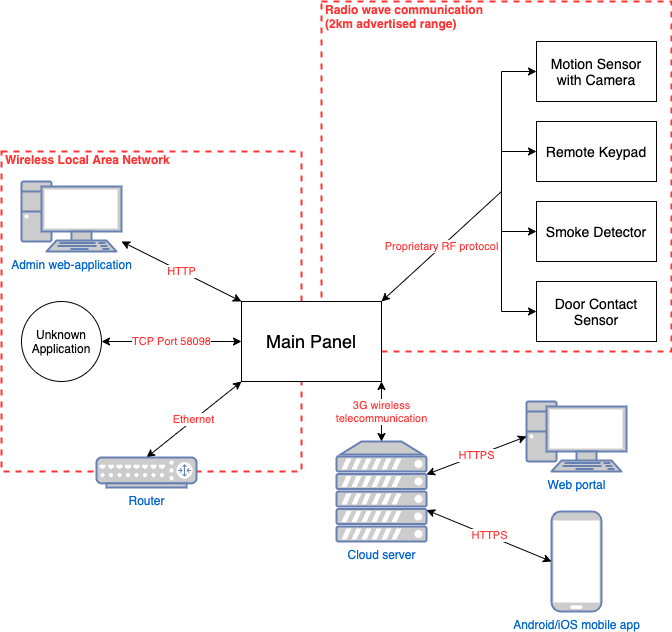
\includegraphics[width=\textwidth]{images/system-overview.png}
    \caption{Overview of the System Architecture}
    \label{fig:system-overview}
\end{figure}

\subsection{System Technologies}
\begin{table}[!ht]
    \centering
    \begin{tabularx}{\textwidth}{l X}
        \textbf{Technology}  & \textbf{Description} \\
        \hline
        Main Panel & Linux 2.6-2.30. Hosts a web server over HTTP, using Mongoose (an embedded web server), version unknown. Unknown application listening on TCP port 58098. Hosts DNS on TCP/UDP port 53. Has a USB and ethernet port. \\
        \hline
        HTTP  & Protocol used by the admin web application. A clear text protocol, used to communicate with the web admin panel. \\
        \hline
        F1 RF protocol  & A proprietary \gls{RF} protocol from the hardware manufacturer, Climax Technology. Uses 868 MHz frequency. Completely undocumented. \\
        \hline
        Mongoose web server  & An open source web server, in C. Used by the main panel to host the local admin web page, version unknown. \\
        \hline
    \end{tabularx}
    \caption{Technologies used in the system}
    \label{tb:system-technologies}
\end{table}

\section{Decomposition of the system}
This section presents the results of the fourth step of the threat modeling technique. Lastly, all identified entry points of the system are listed.

\subsection{Entry points}
\begin{table}[!ht]
    \centering
    \begin{tabularx}{\textwidth}{l X}
        \textbf{Entry point} & \textbf{Description}  \\
        \hline
        Local web admin page  & See section \ref{ch:system:software}. Provides very basic functionality but no control over the system. Has an undocumented login page via \textit{HTTP Basic Auth}. Data is transferred over HTTP on the local network. \\
        Unknown application  & This is a completely undocumented process, listening on TCP port 58098. Closes the connection when sent data. Becomes unresponsive when sent certain data like \texttt{[]} and \texttt{\{\}} (presumably it crashes). \\
        Main panel  & The physical device features an Ethernet port to connect to the local network, as well as a USB port for unknown purposes. It communicates with other devices over a 868 GHz proprietary \gls{RF} protocol. \\
        3G telecommunication  & The device has a SIM-card and communicates over the 3G telecommunication network. \\
        \gls{RF} communication  & The device talks to the other peripherals over a proprietary \gls{RF} protocol, called \textit{F1}\footnotelink{https://www.climax.com.tw/new/f1-features-new.php}{2021-04-02}. There seems to be little to no information available to the public about this protocol, other than it's operating frequency of 868 GHz. \\
        USB port  & The device has a USB 2.0 Type-A connector. \\
        Firmware  & The firmware of the system. \\
        \hline
    \end{tabularx}
    \caption{The entry points of the main panel}
    \label{tb:system-entry-points}
\end{table}